 !Rnw root = AABase.Rnw

\chapter*{Introduction}
\addcontentsline{toc}{chapter}{Introduction}

Welcome to \textbf{Advanced Analytics Using R}: Navingating Business Big Data with R. Let's get started.

\section*{Who Is This Book For?}

This book is for business students, practitioners and executives who want to have hands-on experience in working with business related big data and want to extract actionable insights from the data using advanced analytical techniques. This book is application oriented and hence focuses on the application of advanced analytical techniques rather than the theoretical details. Consequently, this book is not for readers solely focused on the theoretical, statistical part of data analytics. 

This book assumes that the readers have basic familiarity with introductory probability and statistics. This domain is easier to follow and understand if the reader also has \textit{some} exposure to some kind of computer programming although that is not a necessity. This book has been written for a practitioner audience, not an academic one. The book aims to be an exhaustive reference resource for practitioners - that's why it starts with baby steps of introducing R and basic data manipulation and ends at the other end with advanced Machine Learning algorithms and complex model improvement algorithms.

Thank you for placing your trust in this book. This chapter will provider further details about this book and how to best read/use this book.

\section*{About This Document}

This document, which you are probably seeing as a PDF document or an eBook or even a printed book, has been written entirely using R and RStudio. It uses two R packages \rpackage{Sweave} and \rpackage{knitr} to integrated R code inside my favorite document creation system called \LaTeX. This document has been created entirely using Open Source tools and has been released back into the Open Source ecosystem for free using the GNU General Public License (GPL). You are free to share this document with others as long as you comply with the GPL license. \mnote{GPL License usually require that the product (in this case, this book) be made available free or charge; and any subsequent product made using the GPL Licensed product must also be made available free of charge \citep{TheGNUGe51:online}.}

This is my first attempt at writing a book size document. I have had to develop a bunch of \LaTeX, knitr and R workarounds to make the process work and get a quality output. My \LaTeX  template for this book and details of several of the workarounds are posted on my personal website \url{http://ateachr.com}. \mnote{I plan to publish these and other details on ateachr.com - but as of this version of the document, I have not been able to. I will revise this note after I have published the material.}

\section*{Associated R Package and Website}

This book makes use of several data sources, custom developed R code, question sets, documentation and so on. All of these material are packaged together in an R package hosted on GitHub called \rpackage{clarifyR}.\mnote{I think the name is clever. I was pretty happy with myself when I found out that the clarifyR name was available. :-)} You can download all the material associated with the book by installing the clarifyR package in your R installation. For downloading and installing R packages from GitHub, you will need the \rpackage{devtools} package. Follow the code below that uses the following commands: \rcommand{install.packages} for installing a R package, \rcommand{library} for loading a package into memory and finally the \rcommand{install\_github} command that is part of the devtools package for installing a package from GitHub. Note that the install\_github command uses the name of the package and the GitHub username that the package belongs to. As most GitHub packages are public, we do not need a password.


\begin{Schunk}
\begin{Sinput}
> #Code to be changed 
> #Installing clarifyR package from GitHub
> #First get devtools package and load into memory
> install.packages("devtools");library(devtools)
> install_github("clarifyr", username="clarifyr")
> library(clarifyr)
\end{Sinput}
\end{Schunk}

If you wish to access the book contents outside of the R ecosystem, then you can head on to \url{http://clarifyr.com}. The website has all the material available as part of the clarifyR package. The website also works as an interaction platform between the author and readers and students. Feel free to ask any questions related to the book content there - I will be happy to answer them. 

\section*{How is This Book Structured}

This book covers a wide range of material. The material is organized in 5 parts, 19 chapters and several appendices.

\subsection{Part I: Getting Started}

We set ourselves for the book - download and install all needed software; figure our way around R and RStudio and learn the basics of the R language. Essentially lay down enough of a foundation that we can start getting productive. For students without a computer programming background, it is essential that they do not rush this part. Our success in later parts depend upon us getting comfortable with the material here.

\subsection{Part II: Data Exploration and Visualization}

Real data analytics begins with us understanding and getting a handle on the data. This typically involves cleaning up the data,\mnote{In my opinion, data cleaning is the most under-appreciated part of data analytics. It often takes more time and effort than the actual analysis that follows.} generating descriptive statistics to better understand the data and finally creating visualizations that allow us to better understand the underlying complexity of the data.

Data visualization has emerged as a key tool in Big Data Analytics. In this book we devote just one chapter to it - a necessary limitation as we have such a broad variety of topics to cover in this book. We focus our attention here on a subset of data visualization that is important in the business context - creating data dashboards that can help managerial decision making.   

\subsection{Part III: Traditional Statistical Modeling}

Even advanced analytic techniques like machine learning algorithms in the next part have their foundations in traditional statistical methodologies. Classical statistical modeling approaches like Linear Regression are still the benchmark given their immense popularity, flexibility and stability. In this part of the book, we explore traditional statistical analysis tools like Linear Regression, Generalized Linear Models like Logistic and Survival Models, Principal Components and Factor Analysis, Time Series Analysis and so on.

As we assume that you are already familiar with basic probability and statistics, we will focus on application of the methodologies and not the underlying theory. We will also focus on how to tweak these tools for the Big Data world as many of these tools run into trouble when sample sizes are quite large. Bigger is not always better - traditional statisticall methodologies were developed/optimized for smaller sample sizes. Using them for large sample sizes give rise to unique issues and problems - we will discuss how to address them.

\subsection{Part IV: Machine Learning and Predictive Analytics}

This is the largest and the most important part of the book. This is why this book was written in the first place - an overview of data analytics tools specific to Big Data - variously known as Machine Learning, Statistical Learning, Predictive Analytics, Data Mining as so on. This book focuses on tools that help us make sense of Big Data and helps us automate the extraction of managerial decision making insights from Big Data.

As with much of the rest of the book, the focus is on applying the tools rather than their theoretical/mathematical underpinnings. We will discuss enough theory to develop an overall understanding and then devote our energies on making these tools work on real datasets.

\subsection{Part V: Putting It All Together}

Now that we have gone through all the elements individually, we can move forward to create a combined, integrated approach that puts all these pieces together. How to combine different models so that they result in an output better than sum of their parts? How to ensure that our models improve as more data become available? 

We will conclude by running a couple of large integrated data analytics projects that will combine elements discussed in the book. 

\subsection{Part V: Appendices, Bibliography and Index}

Back matter of the book. The Index in the end has three main components - Key Concepts, R Commands and R Packages. Appendices include syllabus for the two courses this book is primarily used for and other miscellaneous content that did not fit in one of the main matter chapters.

There are a lot of quality, free, online resources available for building up your R and Data Analytics skills before you go through this book or the associated courses. They are listed in Appendix: Key References. A fully fleshed data analysis example has been presented on Appendix: Data Analysis Example to give you an idea of the power and range of what can be accomplished with just a little bit of familiarity with R.

\section*{How to Read This Book}

You would have noticed by now that this book integrates R code within its text. Most of the time R code takes the form of dedicated code blocks like the one below:  

\begin{Schunk}
\begin{Sinput}
> #This is a demo code block
> print("Hello World")
\end{Sinput}
\begin{Soutput}
[1] "Hello World"
\end{Soutput}
\end{Schunk}

As you can see from above, code blocks are printed in color, in \texttt{fixed width font}. There is a color scheme here that you will soon become familiar with - comments are in italics and kind of violet looking, functions are in reddish color, strings appear bluish and so on. The output of the code block appears right after - for example - the output of the \rcommand{print} command follows the code above.

You would notice that whenever we refer to a R command in a significant way (like \texttt{print} in paragraph above), the command is printed in \colorbox{yellow}{\texttt{fixed width font}}, in red color with a yellow highlight that makes it easy for you to see which commands are discussed significantly on the page. The highlighting also ensures that an entry for the command is placed in the R Commands section of the Index provided at the end of the book. For times when a command is mentioned in text in a minor way not necessating a margin and Index entry, they will be typed in \texttt{fixed width font}.

Like R Commands, this book provides special formatting for R Packages used in the book. R Packages are fomatted like R Commands but in blue color - check our reference of the \texttt{clarifyR} package earlier - blue fixed width font text with yellow highlighting  and finally an entry in the Packages section of the Index. 

Lastly, special formatting is provided for key concepts - similar to R Commands and Packages in all respects except that they are in bolded and in black color\mnote{\color{green}I would have liked to make margin notes green - but somehow green color prints a horribly toxic green - so I am defaulting to black until I can find a way to print a darker, pleasanter green.} and their Index entry is in the Key Concepts section. For example: this book focuses on \rconcept{Open Source} software - that are created by a community of software developers for use by the community, usually made available for free. 

The three special formatting elements - commands, packages and key concepts - ensure that you have a summary of significant elements discussed in the page just by looking for highlighted items. Other than these, you would also notice that the book makes extensive use of margin notes aligned to the relevant location on the page.\mnote{This is a demo margin note. You will find helpful hints, debugging tips and other thoughts and trivia here.} I use these margin notes for interesting tidbits that I want to emphasize, my tangential thoughts or just stuff I couldn't find space for in the main text. I also expect that the expanded margin area will be useful for readers to make notes, include remarks etc. 

\section*{Important Note on Figure Placements and Other Quirks of \LaTeX}

This book has tonnes of figures - including images and tables. In a book of this size, its quite an undertaking to ensure that all figures are placed appropriately. I typically let \LaTeX\ place figures where it should be placed given considerations of page break, whitespace and readability. This sometimes results in figures being placed a little earlier or later in the document than where you would expect them. Typically \LaTeX\ prefers to put images at the top of the page. I have taken care to refer to figures with their numbering so that you can always identify which figure I am referring to - for exampple - see Figure: \ref{fig:woodson} for my most favorite moment in Michigan Football history - Woodson making an amazing one handed interception against the little brothers. As you can see - the placement is weird. Figure numbers help - still, figure placements in this book can be a little disorienting at first - I hope you will get used to it quickly.

\begin{figure}
\rule{4in}{1pt}
\centering
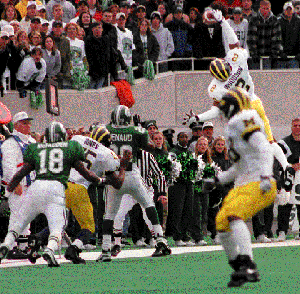
\includegraphics[height=4in]{images/woodson.png}
\caption{Woodson is a Super Human}
\label{fig:woodson}
\rule{4in}{1pt}
\end{figure}

Figures are usually horizontly centered on the page with horizontal lines at the top and botton separting it from the main text. All figures have a figure number and a caption attached to them. All figures are referred in the List of Figures by their figure number, caption text and the page number where they appear. 

This book has been formatted to show page numbers in the bottom center of the page, chapter number and name on the top header of even pages and section number and name on the top header of odd pages. Default font size for this book is 11 points. Contact the author if you would like to get a copy of the PDF version of the book with a larger font size. The original \LaTeX\ files are available upon request as well.

If you would like to know more about \LaTeX\ then I would recommend taking a look through \citet{latexcompanion}. A great, free, online resource to start learning about \LaTeX\ is https://en.wikibooks.org/wiki/LaTeX \citep{LaTeXWik0:online}.

\section*{Is This Book Suitable For You?}

Well - you wouldn't know until you spend some time with it. However, to give you a quick flavor of what you can expect from this book, I have included a sample basic data analysis example in Appendix B. If the material in Appendix B catches your fancy, looks interesting - then you are in the right place. Dig in. 

A quick word of caution though before you get too deep: this book (and the associated courses) are very hands-on. There is no point in reading this book like a sequence of text. This book should be seen more as an illustrated text - illustrated with relevant R commands and material. You should read this book alongside an RStudio session - trying all the commands there as you read along. You will need to get comfortable with a lot of command line typing, keyboard shortcuts and figuring workarounds to inevitable problems that will arise. We will often get into situations where there will be no tested/optimized/prescribed solution and we will need to figure our way out - often with some trial and error. You should be comfortable with such ambiguity.

\chapterendsymbol
